%%%%%%%%%%%%%%%%%%%%%%%%%%%%%%%%%%%%%%%%%%%%%%%%%%%%%%%%%%%%%%%%%%%%%%%%%%%%%%%%%%%%%
%%%%%%%%%%%%%%%%%%%%%%%%%%%%%%%%%%%%%%%%%%%%%%%%%%%%%%%%%%%%%%%%%%%%%%%%%%%%%%%%%%%%%

\setbeamercolor{block title}{bg=white, fg=black}
\setbeamercolor{body}{bg=blue!20}

%%%%%%%%%%%%%%%%%%%%%%%%%%%%%%%%%%%%%%%%%%%%%%%%%%%%%%%%%%%%%%%%%%%%%%%%%%%%%%%%%%%%%
%%%%%%%%%%%%%%%%%%%%%%%%%%%%%%%%%%%%%%%%%%%%%%%%%%%%%%%%%%%%%%%%%%%%%%%%%%%%%%%%%%%%%

\begin{frame}
	\frametitle{Этапы исправления ошибки в программном коде}
	\begin{itemize}
		\item Воспроизведение
		\item \textbf{Локализация}
		\item Изучение
		\item Исправление
		\item Тестирование
	\end{itemize}
\end{frame}

%%%%%%%%%%%%%%%%%%%%%%%%%%%%%%%%%%%%%%%%%%%%%%%%%%%%%%%%%%%%%%%%%%%%%%%%%%%%%%%%%%%%%
%%%%%%%%%%%%%%%%%%%%%%%%%%%%%%%%%%%%%%%%%%%%%%%%%%%%%%%%%%%%%%%%%%%%%%%%%%%%%%%%%%%%%


\begin{frame}[fragile]
	\frametitle{Пример}
	GCC ломается на следующем файле:
	\begin{lstlisting}[style =crs_cpp]
extern int printf (const char *, ...);
static char
(safe_unary_minus_func_int8_t_s)(char si )
{
  return
    (si==(-128)) ?
    ((si)) : -si;
  ...
  2683 lines of code
\end{lstlisting}
\end{frame}


%%%%%%%%%%%%%%%%%%%%%%%%%%%%%%%%%%%%%%%%%%%%%%%%%%%%%%%%%%%%%%%%%%%%%%%%%%%%%%%%%%%%%
%%%%%%%%%%%%%%%%%%%%%%%%%%%%%%%%%%%%%%%%%%%%%%%%%%%%%%%%%%%%%%%%%%%%%%%%%%%%%%%%%%%%%

\begin{frame}
	\small
	\frametitle{Классический дельта-дебаггинг}
	Дано: $test$ и $c_x$, такие что $test(c_x) = fail$ \\
	Необходимо найти: $c'_x = ddmin(c_x)$, такое что $c'_x \subseteq c_x, test(c'_x) = fail$ \\
	\begin{itemize}
		\item Тестовая выборка делится на n частей: $\Delta_1, \Delta_2, ..., \Delta_n$
		\item Формируется остальная часть выборки без $\Delta_i$: $\nabla_i = c_x - \Delta_i$
	\end{itemize}
	Производится тестирование на каждой подвыборке:
	\begin{itemize}
		\item происходит сбой на подвыборке $\Delta_i$: $c_x = \Delta_i$, $n = 2$
		\item происходит сбой на подвыборке $\nabla_i$: $c_x = \nabla_i$, $n = n - 1$
		\item если никакая из подвыборок не приводит к сбою, то $n = 2n$, когда $2n > |c_x|$
	\end{itemize}
\end{frame}

%%%%%%%%%%%%%%%%%%%%%%%%%%%%%%%%%%%%%%%%%%%%%%%%%%%%%%%%%%%%%%%%%%%%%%%%%%%%%%%%%%%%%
%%%%%%%%%%%%%%%%%%%%%%%%%%%%%%%%%%%%%%%%%%%%%%%%%%%%%%%%%%%%%%%%%%%%%%%%%%%%%%%%%%%%%
\definecolor{forest}{rgb}{0,0.7,0}

\begin{frame}[fragile]
	\frametitle{Пример}
\begin{minipage}[t]{0.48\linewidth}
		\begin{itemize}
		\item[] \{1, 2, 3, 4, 5, 6, 6, 8\} 
		\item[] \{1, 2, 3, 4\}			  
		\item[] \{5, 6, 6, 8\}
		\item[] \{5, 6\}
		\item[] \{6, 8\}
		\item[] \{5\}, \{6\}, \{6\}, \{8\}
		\item[] \{5, 6, 6\}
		\item[] \{5, 6\}
		\item[] \{6, 6\}
		\item[] \{6\}
		\item[] \{6\}
		\item[] \textbf{\{6, 6\}}
	\end{itemize}
\end{minipage}
\begin{minipage}[t]{0.48\linewidth}
		\begin{itemize}
		\item[] {\color{red}X}
		\item[] {\color{forest}V}	  
		\item[] {\color{red}X}
		\item[] {\color{forest}V}
		\item[] {\color{forest}V}
		\item[] {\color{forest}V}
		\item[] {\color{red}X}
		\item[] {\color{forest}V}
		\item[] {\color{red}X}
		\item[] {\color{forest}V}
		\item[] {\color{forest}V}
		\item[] {\color{red}X}
	\end{itemize}
\end{minipage}

\end{frame}

%%%%%%%%%%%%%%%%%%%%%%%%%%%%%%%%%%%%%%%%%%%%%%%%%%%%%%%%%%%%%%%%%%%%%%%%%%%%%%%%%%%%%
%%%%%%%%%%%%%%%%%%%%%%%%%%%%%%%%%%%%%%%%%%%%%%%%%%%%%%%%%%%%%%%%%%%%%%%%%%%%%%%%%%%%%

\begin{frame}[fragile]
	\frametitle{``Простой'' дельта-дебаггинг}
	\begin{itemize}
		\item Работает на уровне строк
		\item Не учитывает структуру кода
	\end{itemize}
	\begin{lstlisting}[style=crs_cpp]
void f() {
    int x;
    int y;
    if (x != 0) {
        y = x;
    } else {
        return 0;
    }
    while (y != 0) {
        y--;
    }
    return y;
}
\end{lstlisting}
\end{frame}

%%%%%%%%%%%%%%%%%%%%%%%%%%%%%%%%%%%%%%%%%%%%%%%%%%%%%%%%%%%%%%%%%%%%%%%%%%%%%%%%%%%%%
%%%%%%%%%%%%%%%%%%%%%%%%%%%%%%%%%%%%%%%%%%%%%%%%%%%%%%%%%%%%%%%%%%%%%%%%%%%%%%%%%%%%%
\lstset{escapeinside={<@}{@>}}
\begin{frame}[fragile]
	\frametitle{Дельта-дебаггинг + topformflat}
	\begin{minipage}{0.4\linewidth}
	\begin{figure}
	\resizebox{1.2\linewidth}{!}{%
\begin{tabular}{ |c|c|c| } 
\hline
\bf Код & \bf Глубина  \\
\hline
\tt
\multirow{7}{18em}{int gcd (int a, int b) \{ \\
\ \ \ \ if (b == 0) \{ \\
\ \ \ \ \ \ \ \ return a; \\
\ \ \ \ \} else \{ \\
\ \ \ \ \ \ \ \ return gcd (b, a \% b); \\
\ \ \ \ \} \\
\}
} & 0\\ 
& 1 \\ 
& 2  \\ 
& 1 \\ 
& 2  \\ 
& 1 \\ 
& 0 \\
\hline
\end{tabular}}
	\end{figure}
	\end{minipage}
	\begin{minipage}{0.1\linewidth}
	\ \ 
	\end{minipage}
	\begin{minipage}{0.4\linewidth}
		\begin{figure}
		\resizebox{1.3\linewidth}{!}{%
\begin{tabular}{ |c|c|c| } 
\hline
\bf Код & \bf Глубина  \\
\hline
\tt
\multirow{4}{22em}{int gcd (int a, int b) \{ \\
\ \ \ \ if (b == 0) \{ return a; \} \\
\ \ \ \ else \{ return gcd (b, a \% b); \} \\
\}
} & 0\\ 
& 1 \\ 
& 1  \\ 
& 0 \\
\hline
\end{tabular}}
	\end{figure}
	\end{minipage}
	\\ \
	\center{ 
	Подходит для ограниченного числа языков в ограниченном количестве случаев}
\end{frame}

%%%%%%%%%%%%%%%%%%%%%%%%%%%%%%%%%%%%%%%%%%%%%%%%%%%%%%%%%%%%%%%%%%%%%%%%%%%%%%%%%%%%%
%%%%%%%%%%%%%%%%%%%%%%%%%%%%%%%%%%%%%%%%%%%%%%%%%%%%%%%%%%%%%%%%%%%%%%%%%%%%%%%%%%%%%

\begin{frame}
	\frametitle{Иерархический дельта-дебаггинг}
	Алгоритм дельта-дебаггинга применяется к синтаксическому дереву, представляющему входной тест \\ \ \\
	Алгоритм иерархического дельта-дебаггинга:
	\begin{algorithmic}
		\State $level \gets 0$
		\State $node \gets getNodesOfLevel(tree, 0)$
		\State while$(nodes \neq \emptyset)$ do
		\State \ \ \ \ $minconfig \gets DDMIN(nodes)$
		\State \ \ \ \ $delete(tree, level, minconfig)$
		\State \ \ \ \ $level \gets level + 1$
		\State \ \ \ \ $nodes \gets getNodesOfLevel(tree, level)$
		\State $end while$
		
	\end{algorithmic}
\end{frame}


%%%%%%%%%%%%%%%%%%%%%%%%%%%%%%%%%%%%%%%%%%%%%%%%%%%%%%%%%%%%%%%%%%%%%%%%%%%%%%%%%%%%%
%%%%%%%%%%%%%%%%%%%%%%%%%%%%%%%%%%%%%%%%%%%%%%%%%%%%%%%%%%%%%%%%%%%%%%%%%%%%%%%%%%%%%

\begin{frame}
	\frametitle{Иерархический дельта-дебаггинг}
	\begin{figure}
		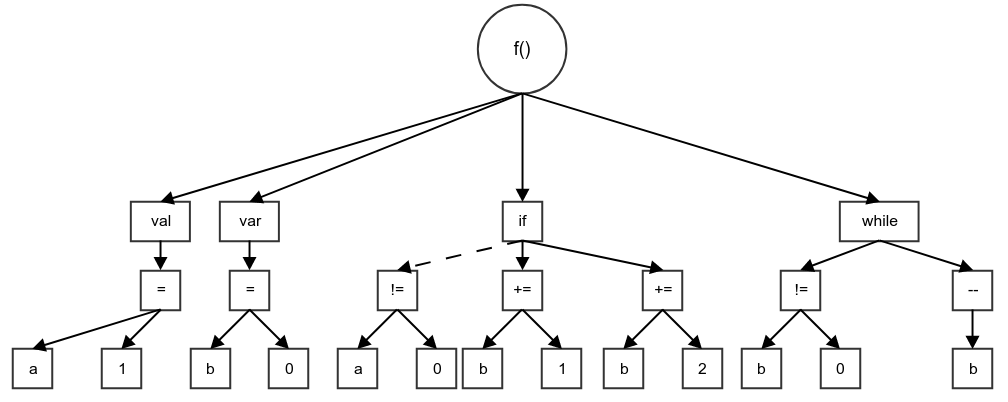
\includegraphics[width=100mm]{image/hddexample}
	\end{figure}	
\end{frame}

%%%%%%%%%%%%%%%%%%%%%%%%%%%%%%%%%%%%%%%%%%%%%%%%%%%%%%%%%%%%%%%%%%%%%%%%%%%%%%%%%%%%%
%%%%%%%%%%%%%%%%%%%%%%%%%%%%%%%%%%%%%%%%%%%%%%%%%%%%%%%%%%%%%%%%%%%%%%%%%%%%%%%%%%%%%

\begin{frame}
	\frametitle{Иерархический-дельта дебаггинг}
	\begin{figure}
		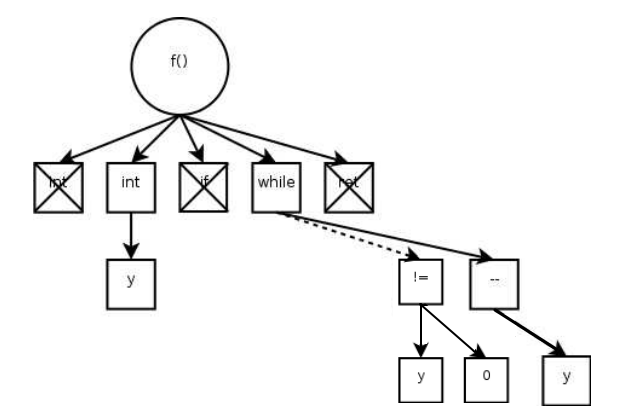
\includegraphics[width=100mm]{image/hdd}
	\end{figure}	
\end{frame}

%%%%%%%%%%%%%%%%%%%%%%%%%%%%%%%%%%%%%%%%%%%%%%%%%%%%%%%%%%%%%%%%%%%%%%%%%%%%%%%%%%%%%
%%%%%%%%%%%%%%%%%%%%%%%%%%%%%%%%%%%%%%%%%%%%%%%%%%%%%%%%%%%%%%%%%%%%%%%%%%%%%%%%%%%%%

\begin{frame}[fragile]
	\frametitle{Слайсинг}
		Slicing (слайсинг) --- выделение из программы ее определенных частей. \\ \
	\small
	\begin{minipage}{0.4\linewidth}
	\begin{lstlisting}[language = pascal]
BEGIN
READ(X,Y)
TOTAL := 0.0
SUM := 0.0
IF X <= 1
    THEN SUM := Y
    ELSE BEGIN
        READ(Z)
        TOTAL := X*Y
    END
WRITE(TOTAL, SUM)
END.
\end{lstlisting}
	\end{minipage}
	\begin{minipage}{0.1\linewidth}
	\ \ 
	\end{minipage}
	\begin{minipage}{0.4\linewidth}
\begin{lstlisting}[language = pascal]
BEGIN
READ(X,Y)
TOTAL := 0.0
IF X <= 1
    THEN 
    ELSE TOTAL := X*Y
END.
\end{lstlisting}
	\end{minipage}
\end{frame}

%%%%%%%%%%%%%%%%%%%%%%%%%%%%%%%%%%%%%%%%%%%%%%%%%%%%%%%%%%%%%%%%%%%%%%%%%%%%%%%%%%%%%
%%%%%%%%%%%%%%%%%%%%%%%%%%%%%%%%%%%%%%%%%%%%%%%%%%%%%%%%%%%%%%%%%%%%%%%%%%%%%%%%%%%%%


\begin{frame}
	\frametitle{Слайсинг}
	Виды слайсинга:
	\begin{itemize}
		\item Прямой и обратный
		\item Статический и динамический
	\end{itemize}
	Плюсы и минусы:
	\begin{itemize}
		\item Скорость и точность работы
		\item Высокая сложность реализации (анализ указателей и учет уровней абстракции для ООП-языков)
	\end{itemize}
	
\end{frame}
	
%%%%%%%%%%%%%%%%%%%%%%%%%%%%%%%%%%%%%%%%%%%%%%%%%%%%%%%%%%%%%%%%%%%%%%%%%%%%%%%%%%%%%
%%%%%%%%%%%%%%%%%%%%%%%%%%%%%%%%%%%%%%%%%%%%%%%%%%%%%%%%%%%%%%%%%%%%%%%%%%%%%%%%%%%%%

\begin{frame}
	\frametitle{Существующие инструменты}
	\begin{itemize}
		\item Picireny
			\begin{itemize}
				\item Иерархический дельта-дебаггер
				\item ANTLR v4 grammar
				\item Критерий
			\end{itemize}
		\item Creduce (Delta)
			\begin{itemize}
				\item Редуктор для языка C
				\item Состоит из набора трансформаций над исходным кодом
				\item 57 компиляторных сбоев
				\begin{itemize}
					\item Delta: 8600 байт
					\item Creduce: 120 байт
				\end{itemize}
			\end{itemize}
		\item JSlice, Indus, JavaBST, CodeSurfer
			\begin{itemize}
				\item Реализуют различные алгоритмы слайсинга для языков Java/C++
			\end{itemize}
	\end{itemize}
	Все приведенные средства работают с языками Java и C++
\end{frame}
%%%%%%%%%%%%%%%%%%%%%%%%%%%%%%%%%%%%%%%%%%%%%%%%%%%%%%%%%%%%%%%%%%%%%%%%%%%%%%%%%%%%%
%%%%%%%%%%%%%%%%%%%%%%%%%%%%%%%%%%%%%%%%%%%%%%%%%%%%%%%%%%%%%%%%%%%%%%%%%%%%%%%%%%%%%

\begin{frame}
	\frametitle{Мотивация}
	\begin{itemize}
		\item Редукция разрабатываемых программ
		\item Существует генератор случайных тестов для компилятора Kotlin
		\item Зачастую компиляторные баги находятся в очень больших проектах
	\end{itemize}
\end{frame}
%%%%%%%%%%%%%%%%%%%%%%%%%%%%%%%%%%%%%%%%%%%%%%%%%%%%%%%%%%%%%%%%%%%%%%%%%%%%%%%%%%%%%
%%%%%%%%%%%%%%%%%%%%%%%%%%%%%%%%%%%%%%%%%%%%%%%%%%%%%%%%%%%%%%%%%%%%%%%%%%%%%%%%%%%%%

\begin{frame}
	\frametitle{Алгоритм редукции}
	\begin{figure}
		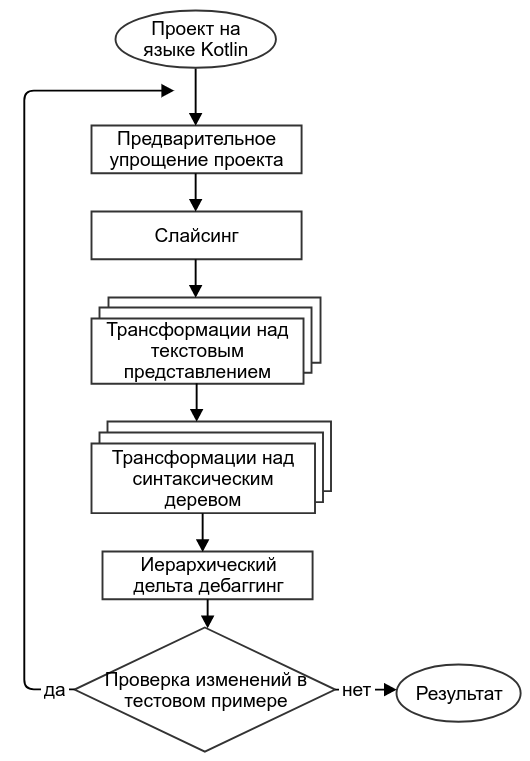
\includegraphics[width=55mm]{image/scheme}
	\end{figure}	
\end{frame}

%%%%%%%%%%%%%%%%%%%%%%%%%%%%%%%%%%%%%%%%%%%%%%%%%%%%%%%%%%%%%%%%%%%%%%%%%%%%%%%%%%%%%
%%%%%%%%%%%%%%%%%%%%%%%%%%%%%%%%%%%%%%%%%%%%%%%%%%%%%%%%%%%%%%%%%%%%%%%%%%%%%%%%%%%%%

\begin{frame}
	\frametitle{Проблема воспроизведения ошибки}
		Часто сообщения об одной и той же ошибке могут сильно различаться. Существуют следующие способы решения проблемы:
		\begin{itemize}
			\item Выделение необходимой информации
			\item Сравнение сообщений об ошибке (разностный алгоритм Майерса)
		\end{itemize}
\end{frame}

%%%%%%%%%%%%%%%%%%%%%%%%%%%%%%%%%%%%%%%%%%%%%%%%%%%%%%%%%%%%%%%%%%%%%%%%%%%%%%%%%%%%%
%%%%%%%%%%%%%%%%%%%%%%%%%%%%%%%%%%%%%%%%%%%%%%%%%%%%%%%%%%%%%%%%%%%%%%%%%%%%%%%%%%%%%

\begin{frame}
	\frametitle{Предварительное упрощение проекта}
		\begin{itemize}
			\item Строится дерево импортирований
			\item Начиная с наибольшей глубины для каждой вершины производится запуск упрощающих трансформаций
				\begin{itemize}
					\item Упрощение функций и свойств
					\item Трансформации над текстовым представлением
					\item Удаление пустых управляющих конструкций
					\item Удаление неиспользуемых импортирований
				\end{itemize}
		\end{itemize}			
\end{frame}

%%%%%%%%%%%%%%%%%%%%%%%%%%%%%%%%%%%%%%%%%%%%%%%%%%%%%%%%%%%%%%%%%%%%%%%%%%%%%%%%%%%%%
%%%%%%%%%%%%%%%%%%%%%%%%%%%%%%%%%%%%%%%%%%%%%%%%%%%%%%%%%%%%%%%%%%%%%%%%%%%%%%%%%%%%%

\begin{frame}
	\frametitle{Слайсинг}
		Программный срез производится на следующих уровнях:
		\begin{itemize}
			\item Уровень классов
			\item Уровень функций
			\item Уровень выражений
		\end{itemize}
\end{frame}

%%%%%%%%%%%%%%%%%%%%%%%%%%%%%%%%%%%%%%%%%%%%%%%%%%%%%%%%%%%%%%%%%%%%%%%%%%%%%%%%%%%%%
%%%%%%%%%%%%%%%%%%%%%%%%%%%%%%%%%%%%%%%%%%%%%%%%%%%%%%%%%%%%%%%%%%%%%%%%%%%%%%%%%%%%%

\begin{frame}
	\frametitle{Трансформации над текстовым представлением}
		Сформирован следующий набор трансформаций над текстовым представлением:
		\begin{itemize}
			\item Удаление текста внутри сбалансированной пары скобок
			\item Замена текста
			\begin{itemize}
				\item замена текста, подходящего под шаблон, например, <<1294>> на~<<0>>; 
				\item замена части текста, подходящего под шаблон, на другой, например <<\texttt{i = i + 1}>> на~<<\texttt{i++}>>;
				\item применение к тексту, подходящему под шаблон, другого шаблона, например <<\texttt{a + b + c + d}>> преобразуется в~<<\texttt{a + b}>>.
\end{itemize}
		\end{itemize}
\end{frame}

%%%%%%%%%%%%%%%%%%%%%%%%%%%%%%%%%%%%%%%%%%%%%%%%%%%%%%%%%%%%%%%%%%%%%%%%%%%%%%%%%%%%%
%%%%%%%%%%%%%%%%%%%%%%%%%%%%%%%%%%%%%%%%%%%%%%%%%%%%%%%%%%%%%%%%%%%%%%%%%%%%%%%%%%%%%

\begin{frame}
	\frametitle{Трансформации над синтаксическим деревом}
		\small
		Сформирован следующий набор трансформаций над синтаксическим деревом:
		\footnotesize
		\begin{itemize}
			\item Упрощение операторов
				\begin{itemize}
				\footnotesize
					\item элвис
					\item if
					\item ...
				\end{itemize}
			\item Удаление неиспользуемых компонентов
				\begin{itemize}
				\footnotesize
					\item аргументов функций
					\item аргументов конструктора
					\item ...
				\end{itemize}
			\item Упрощение внутренних связей
				\begin{itemize}
				\footnotesize
					\item Удаление унаследованных свойств и функций
					\item Замена тел функций на вызов TODO()
					\item ...
				\end{itemize}
			\item Другие
				\begin{itemize}
					\footnotesize
					\item Удаление комментариев
					\item Замена возвращаемого значения функции
					\item ...
				\end{itemize}
		\end{itemize}				
\end{frame}


%%%%%%%%%%%%%%%%%%%%%%%%%%%%%%%%%%%%%%%%%%%%%%%%%%%%%%%%%%%%%%%%%%%%%%%%%%%%%%%%%%%%%
%%%%%%%%%%%%%%%%%%%%%%%%%%%%%%%%%%%%%%%%%%%%%%%%%%%%%%%%%%%%%%%%%%%%%%%%%%%%%%%%%%%%%

\begin{frame}
	\frametitle{Иерархический дельта дебаггинг}
		\begin{itemize}
			\item Иерархический дельта дебаггинг является заключительной трансформацией
			\item К каждому уровню дерева, начиная с верхнего, применяется алгоритм классического дельта дебаггинга
			\item Данная трансформация может порождать синтаксически некорректный код
		\end{itemize}
\end{frame}
%%%%%%%%%%%%%%%%%%%%%%%%%%%%%%%%%%%%%%%%%%%%%%%%%%%%%%%%%%%%%%%%%%%%%%%%%%%%%%%%%%%%%
%%%%%%%%%%%%%%%%%%%%%%%%%%%%%%%%%%%%%%%%%%%%%%%%%%%%%%%%%%%%%%%%%%%%%%%%%%%%%%%%%%%%%

\begin{frame}[fragile]
	На основе предложенного метода быд разработан прототип:
		\begin{itemize}
			\item Основное предназначение --- редукция компиляторных тестов
			\item Для ускорения работы некоторые трансформации работают параллельно
			\item Для обеспечения безопасности после применения любой трансформации производится проверка воспроизведения ошибки
		\end{itemize}
\end{frame}
%%%%%%%%%%%%%%%%%%%%%%%%%%%%%%%%%%%%%%%%%%%%%%%%%%%%%%%%%%%%%%%%%%%%%%%%%%%%%%%%%%%%%
%%%%%%%%%%%%%%%%%%%%%%%%%%%%%%%%%%%%%%%%%%%%%%%%%%%%%%%%%%%%%%%%%%%%%%%%%%%%%%%%%%%%%

\begin{frame}[fragile]
	\frametitle{Результаты тестирования}
\begin{table}[]
\center
\footnotesize
\begin{tabular}{| c | c | c |}
\hline
\bf Название & \bf N строк, тыс. & \bf Размер файла с ошибкой, Кб \\
\hline
compTests & 9 & 198.7\\
\hline
kotlinpoet & 10 & 15.2\\
\hline
kfg & 3.5 & 40.2\\
\hline
mapdb & 2 & 12.5\\
\hline
kotoed & 20 & 24\\
\hline
\end{tabular}
\end{table}

\begin{table}[]
\footnotesize
\begin{tabular}{| c | c | c | c | c | c | c |}
\hline
\bf \multirow{2}{*}{Проект} & \multicolumn{2}{|c|}{\bf Slice} & \multicolumn{2}{|c|}{\bf HDD} & \multicolumn{2}{|c|}{\bf Full} \\
\cline{2-7}
& время & размер & время & размер & время & размер \\
\hline
compTests & 2:30 & 65.6 & 32:23 & 33.9 & 31:55 & 21.6 \\
\hline
kotlinpoet & 2:35 & 15.1 & 80:10 & 1.8 & 16:15 & 0.3 \\
\hline
kfg & 5:29 & 38.9 & 769:19 & 1.0 & 18:48 & 0.04 \\
\hline
mapdb & 1:23 & 7.2 & 21:22 & 2.2 & 2:55 & 0.04 \\
\hline
kotoed & 9:50 & 16.4 & 971:51 & 5.5 & 61:00 & 0.8 \\
\hline
\end{tabular}
\end{table}
\end{frame}


%%%%%%%%%%%%%%%%%%%%%%%%%%%%%%%%%%%%%%%%%%%%%%%%%%%%%%%%%%%%%%%%%%%%%%%%%%%%%%%%%%%%%
%%%%%%%%%%%%%%%%%%%%%%%%%%%%%%%%%%%%%%%%%%%%%%%%%%%%%%%%%%%%%%%%%%%%%%%%%%%%%%%%%%%%%

\begin{frame}[fragile]
	\frametitle{Пример работы}
	\begin{lstlisting}[basicstyle=\fontsize{4}{1}\selectfont\ttfamily]
class Outer {
val Outer.outerProp: String
constructor(x: String) {
 outerProp = x
 }

var sideEffects = ""
inner class A1() {
var prop: String = ""

constructor(x: String): this() {
 prop = x + "#${outerProp}"
 sideEffects += "#third"
 }

}
inner class A2 {
var prop: String = ""
init {
 sideEffects += outerProp + "#" + prop + "first"
 }

constructor(x: String) {
 prop = x + "#$outerProp"
 sideEffects += "#third"
 }

init {
 sideEffects += prop + "#second"
 }

constructor(x: Int) {
 prop += "$x#$outerProp#int"
 sideEffects += "#fourth"
 }

}
}
fun box(): String {
val outer1 = Outer("propValue1")
val a1 = outer1.A1("abc")
if (a1.prop != "abc#propValue1") {
return "fail1: ${a1.prop}"
}
if (outer1.sideEffects != "propValue1#first#second#third") {
return "fail1-sideEffects: ${outer1.sideEffects}"
}
val a2 = outer2.A1(123)
if (a2.prop != "123#propValue2#propValue2#int") {
return "fail2: ${a2.prop}"
}
...
100 lines more
\end{lstlisting}
	
\end{frame}

%%%%%%%%%%%%%%%%%%%%%%%%%%%%%%%%%%%%%%%%%%%%%%%%%%%%%%%%%%%%%%%%%%%%%%%%%%%%%%%%%%%%%
%%%%%%%%%%%%%%%%%%%%%%%%%%%%%%%%%%%%%%%%%%%%%%%%%%%%%%%%%%%%%%%%%%%%%%%%%%%%%%%%%%%%%

\begin{frame}[fragile]
	\frametitle{Результат работы}
	\begin{lstlisting}[basicstyle=\small]
class Outer {
    val Outer.outerProp: String

    constructor(x: String) {
        outerProp = x
    }
}
\end{lstlisting}
	
\end{frame}

%%%%%%%%%%%%%%%%%%%%%%%%%%%%%%%%%%%%%%%%%%%%%%%%%%%%%%%%%%%%%%%%%%%%%%%%%%%%%%%%%%%%%
%%%%%%%%%%%%%%%%%%%%%%%%%%%%%%%%%%%%%%%%%%%%%%%%%%%%%%%%%%%%%%%%%%%%%%%%%%%%%%%%%%%%%

\begin{frame}
	\frametitle{Дальнейшее развитие результатов}
	\begin{itemize}
		\item Дополнение и усложнение трансформаций
		\item Реализация более сложных алгоритмов программного среза
		\item Приме­нение технологии машинного обучения для формирования квази­оптимального набора и порядка запуска разработанных трансфор­маций
		\item Усовершенствование кода
	\end{itemize}
\end{frame}


%%%%%%%%%%%%%%%%%%%%%%%%%%%%%%%%%%%%%%%%%%%%%%%%%%%%%%%%%%%%%%%%%%%%%%%%%%%%%%%%%%%%%
%%%%%%%%%%%%%%%%%%%%%%%%%%%%%%%%%%%%%%%%%%%%%%%%%%%%%%%%%%%%%%%%%%%%%%%%%%%%%%%%%%%%%

\begin{frame}[fragile]
\frametitle{Контакты}
\texttt{stepanov@kspt.icc.spbstu.ru} \\ \ \\ \ \\
ReduKtor repository: \texttt{https://bitbucket.org/vorpal-research/reduktor}
\\ \ \\ 
\begin{columns} 
\column{0.33\textwidth} 
	\begin{figure}
		
\includegraphics[width=0.99\linewidth]{image/polytech_logo_en} 
	\end{figure}
\column{0.33\textwidth} 
	\begin{figure}
		
\includegraphics[width=0.99\linewidth]{image/jetbrainsLogo} 
	\end{figure}
\end{columns}
\end{frame}
